%%%%%%%%%%%%%%%%%%%%%%%%%%%%%%%%%%%%%%%%%
% Short Sectioned Assignment
% LaTeX Template
% Version 1.0 (5/5/12)
%
% This template has been downloaded from:
% http://www.LaTeXTemplates.com
%
% Original author:
% Frits Wenneker (http://www.howtotex.com)
%
% License:
% CC BY-NC-SA 3.0 (http://creativecommons.org/licenses/by-nc-sa/3.0/)
%
%%%%%%%%%%%%%%%%%%%%%%%%%%%%%%%%%%%%%%%%%

%----------------------------------------------------------------------------------------
%	PACKAGES AND OTHER DOCUMENT CONFIGURATIONS
%----------------------------------------------------------------------------------------

\documentclass[paper=a4, fontsize=11pt]{scrartcl} % A4 paper and 11pt font size

\usepackage[T1]{fontenc} % Use 8-bit encoding that has 256 glyphs
%\usepackage{fourier} % Use the Adobe Utopia font for the document - comment this line to return to the LaTeX default
\usepackage[english]{babel} % English language/hyphenation
\usepackage{amsmath,amsfonts,amsthm} % Math packages
%\usepackage[version=3]{mhchem} % Package for chemical equation typesetting
\usepackage{siunitx} % Provides the \SI{}{} and \si{} command for typesetting SI units
\usepackage{graphicx} % Required for the inclusion of images
%\usepackage{natbib} % Required to change bibliography style to APA
\usepackage{authblk}
\usepackage{indentfirst}
\usepackage{subcaption}
\usepackage{wrapfig}
\usepackage{multirow}
\usepackage{hyperref}
\usepackage{float}
\usepackage{url}
\usepackage{booktabs}
\usepackage{times}

\usepackage{lipsum} % Used for inserting dummy 'Lorem ipsum' text into the template

\usepackage{sectsty} % Allows customizing section commands
\allsectionsfont{\centering \normalfont\scshape} % Make all sections centered, the default font and small caps

\usepackage{geometry}
\geometry{left=2.5cm,right=2.5cm,top=2.5cm,bottom=2.5cm}

\graphicspath{{images/}{figures/}}

\usepackage{fancyhdr} % Custom headers and footers
\pagestyle{fancyplain} % Makes all pages in the document conform to the custom headers and footers
\fancyhead{} % No page header - if you want one, create it in the same way as the footers below
\fancyfoot[L]{} % Empty left footer
\fancyfoot[C]{} % Empty center footer
\fancyfoot[R]{\thepage} % Page numbering for right footer
\renewcommand{\headrulewidth}{0pt} % Remove header underlines
\renewcommand{\footrulewidth}{0pt} % Remove footer underlines
\setlength{\headheight}{13.6pt} % Customize the height of the header

\numberwithin{equation}{section} % Number equations within sections (i.e. 1.1, 1.2, 2.1, 2.2 instead of 1, 2, 3, 4)
\numberwithin{figure}{section} % Number figures within sections (i.e. 1.1, 1.2, 2.1, 2.2 instead of 1, 2, 3, 4)
\numberwithin{table}{section} % Number tables within sections (i.e. 1.1, 1.2, 2.1, 2.2 instead of 1, 2, 3, 4)

\linespread{1.2}

%\setlength\parindent{0pt} % Removes all indentation from paragraphs - comment this line for an assignment with lots of text

%----------------------------------------------------------------------------------------
%	TITLE SECTION
%----------------------------------------------------------------------------------------

\newcommand{\horrule}[1]{\rule{\linewidth}{#1}} % Create horizontal rule command with 1 argument of height

\title{	
	\normalfont \normalsize 
	\textsc{Philipps-Universitaet Marburg, The Department of Physics} \\ [25pt] % Your university, school and/or department name(s)
	\horrule{0.5pt} \\[0.4cm] % Thin top horizontal rule
	\huge Computational Physics II: Assignment 2 \\ % The assignment title
	\horrule{2pt} \\[0.5cm] % Thick bottom horizontal rule
}

\author{Houchen \textsc{Li}} % Your name

\date{\normalsize\today} % Today's date or a custom date

\begin{document}

\maketitle % Print the title

%----------------------------------------------------------------------------------------
%	PROBLEM 1
%----------------------------------------------------------------------------------------

\section{Random walks}

According to the definition of round function, it has
\begin{gather*}
	P\left( l_n=b,b+a \right)=\frac{1}{2a}.\\
	P\left( l_n=b+1,\cdots,b+a-1 \right)=\frac{1}{a}.
\end{gather*}
since \(l_n=\text{round}\left( a\cdot r_n+b \right)\), where \(r_n\) is a uniform random variable in \( \left( 0,1 \right)\), while \(a\) and \(b\) are integers.\par
Thus the first moment and the second moment can be given out
\begin{align*}
	\left<l_n\right>&=\frac{1}{2a}\cdot b+\frac{1}{a}\left(\sum_{i=b+1}^{b+a-1}i\right)+\frac{1}{2a}\cdot \left(b+a\right)=b+\frac{a}{2}.\\
	\left<l_n^2\right>&=\frac{1}{2a}\cdot b^2+\frac{1}{a}\left(\sum_{i=b+1}^{b+a-1}i^2\right)+\frac{1}{2a}\cdot \left(b+a\right)^2=b\left( b+a \right)+\frac{2a^2+1}{6}.
\end{align*}
Consequently, the diffusion constant \(D\) will be
\begin{equation*}
	D=\left<l_n^2\right>-\left<l_n\right>^2=b\left( b+a \right)+\frac{2a^2+1}{6}-\left( b+\frac{a}{2} \right)^2=\frac{a^2+2}{12}.
\end{equation*}
Then we plot the probability density out, and compare them to the theoretical prediction. It seems the predictions fit the practices very well.\par
\begin{figure}[!htbp]
	\centering
	\begin{subfigure}[b]{0.495\textwidth}
		\centering
		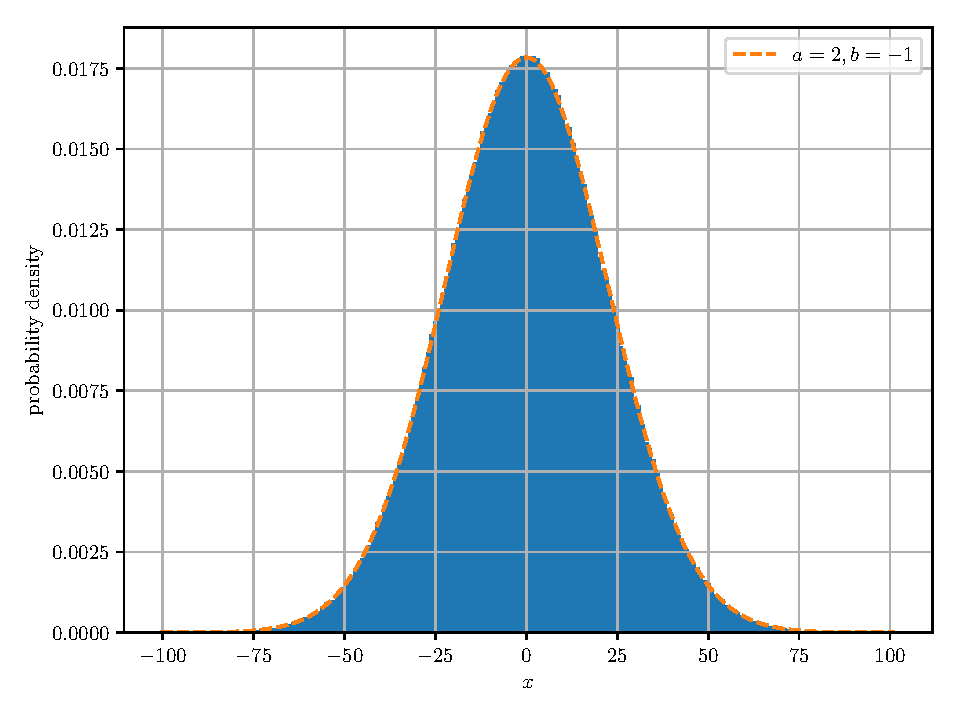
\includegraphics[width=\linewidth]{figure_1_a.pdf}
		\caption{}
	\end{subfigure}
	\begin{subfigure}[b]{0.495\textwidth}
		\centering
		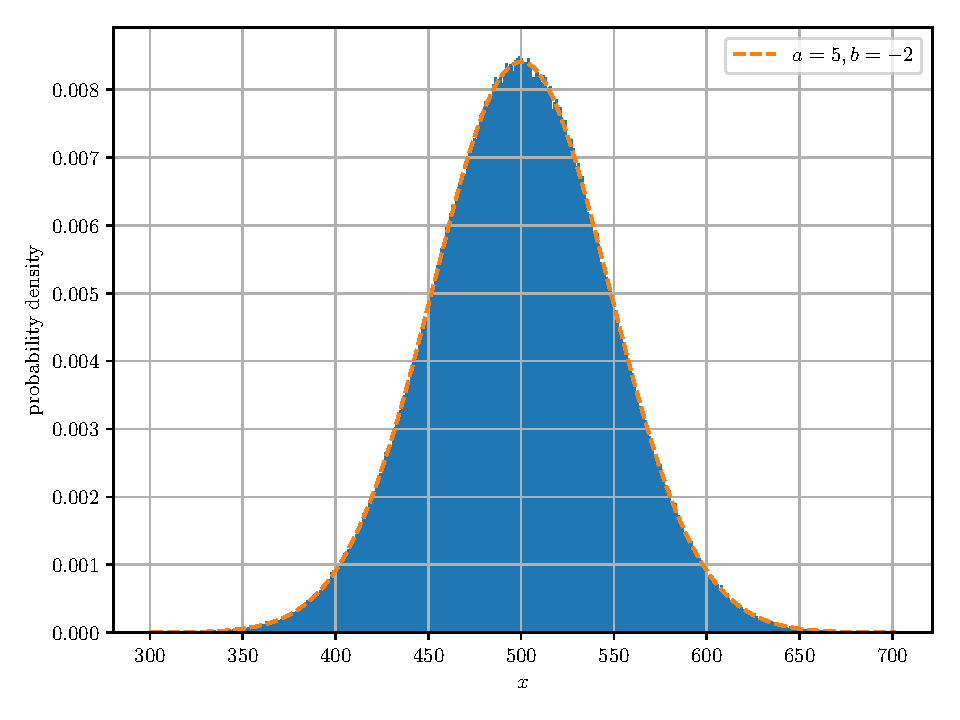
\includegraphics[width=\linewidth]{figure_1_b.pdf}
		\caption{}
	\end{subfigure}
	\caption{the position after 1000 steps: (a) \(a=2,b=-1\); (b) \(a=5,b=-2\).}
	\label{fig:random_1}
\end{figure}
\par

%----------------------------------------------------------------------------------------
%	PROBLEM 2
%----------------------------------------------------------------------------------------

\section{Moments of the normal distribution}

By using Mathematica, the exact results for higher moments
\begin{equation*}
	\left<x^k\right>=\int x^kp\left( x \right)\mathrm{d}x.
\end{equation*}
of Gaussian distribution
\begin{equation*}
	p\left( x \right)=\frac{1}{\sqrt{2\pi\sigma^2}}\exp\left( -\frac{x^2}{2\sigma^2} \right).
\end{equation*}
are determined
\begin{equation*}
	\left<x^k\right>=\begin{cases}0&\text{if \(k\) is odd}\\\left(k-1\right)!!\cdot\sigma^{k}&\text{if \(k\) is even}\end{cases}.
\end{equation*}
Hence, the moments are given out
\begin{table}[!ht]
	\centering
	\caption{The high order moments for Gaussian distribution.}
	\label{tab:moments}
	\begin{tabular}{cccccc}
		\toprule
		\(k\) & 2 & 4 & 6 & 8 & 10 \\
		\midrule
		\(\left<x^k\right>\) & \(\sigma^2\) & \(3\sigma^4\) & \(15\sigma^6\) & \(105\sigma^8\) & \(945\sigma^{10}\)\\
		\bottomrule
	\end{tabular}
\end{table}\par

%----------------------------------------------------------------------------------------
%	PROBLEM 3
%----------------------------------------------------------------------------------------

\section{Parrondos paradoxical games}

I first tried with strategy A and B separately. The probability density function to loss 100 Jetons after specific time steps are presented in Figure~\ref{fig:parrondos_1}, who evident that the separately strategy A or B are both losing games.\par
\begin{figure}[!ht]
	\centering
	\begin{subfigure}[b]{0.495\textwidth}
		\centering
		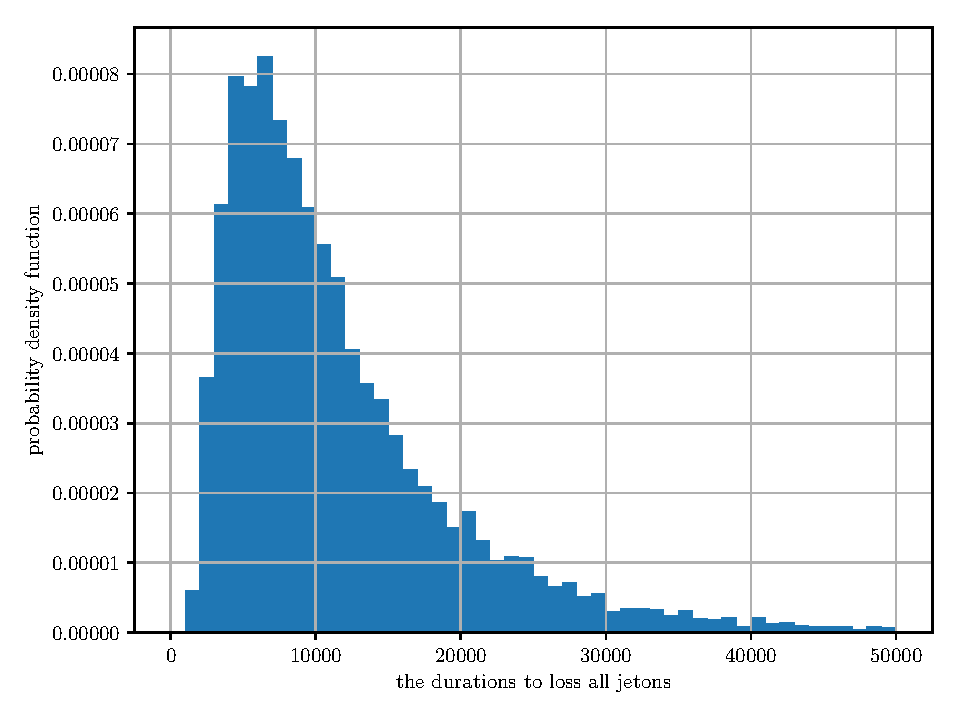
\includegraphics[width=\linewidth]{figure_3_a.pdf}
		\caption{}
	\end{subfigure}
	\begin{subfigure}[b]{0.495\textwidth}
		\centering
		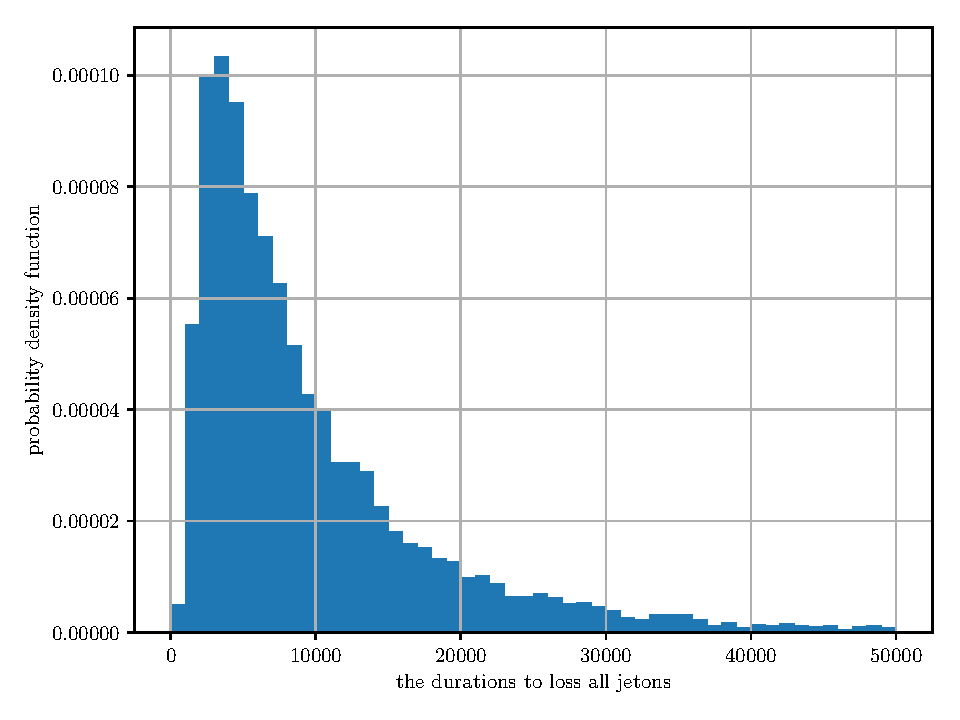
\includegraphics[width=\linewidth]{figure_3_b.pdf}
		\caption{}
	\end{subfigure}
	\caption{the probability to loss 100 Jetons after specific duration: (a) strategy A; (b) strategy B.}
	\label{fig:parrondos_1}
\end{figure}
If I play A and B alternatively, the duration it take to loss 100 Jetons distributes as shown in Figure~\ref{fig:parrondos_2}.\par
\begin{figure}[!ht]
	\centering
	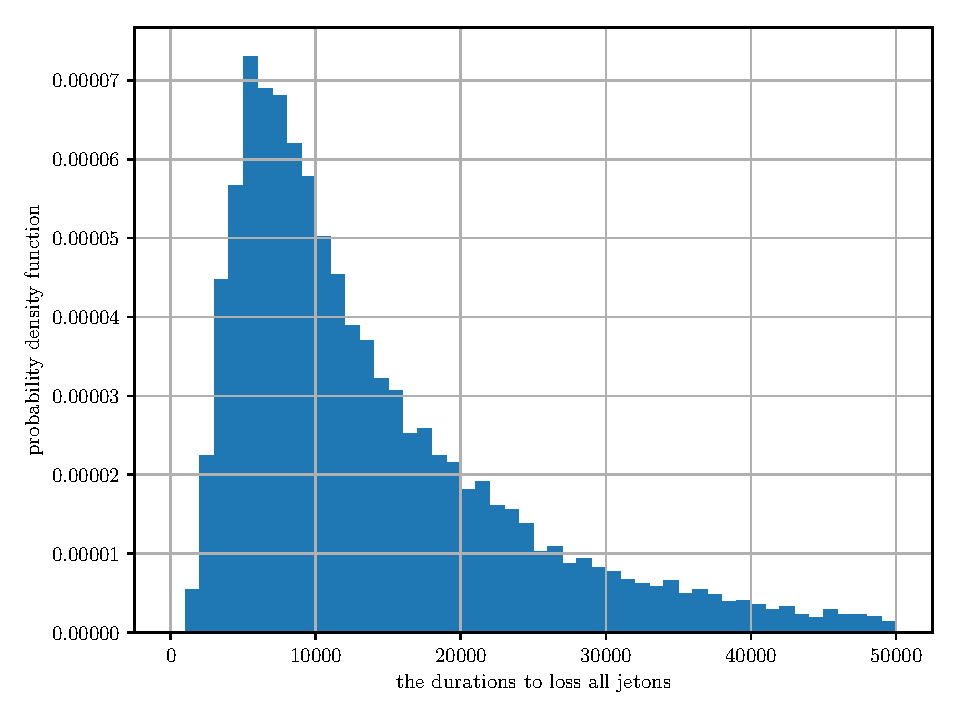
\includegraphics[width=0.5\linewidth]{figure_3_c.pdf}
	\caption{the probability to loss 100 Jetons after specific duration for AB sequence.}
	\label{fig:parrondos_2}
\end{figure}
At last, I tried the sequence AAB. The total amounts of jetons increase from 100 to 50000 very rapidly, which means this kind of playing strategy is a wining games.\par

%----------------------------------------------------------------------------------------

\end{document}
